\section{Decision Trees} 

  In here, we define the decision tree model. It is most natural for classification, but there are variants of it for regression. To avoid confusion, I will distinguish them by calling them classification trees and regression trees, and I will use the umbrella term \textit{decision tree}. 

  Many discriminative models can be written in a clean formula (e.g. $y = w^T x + \epsilon$ for linear regression, and even $y = \prod_i (\sigma_i \circ A_i) (x)$ for MLPs). However, we cannot find such a parameteric form for a tree, which is why they are nonparametric models. In full generality, all we can say is that they have a general tree structure, and there are many variants. 

\subsection{Classification Trees}

  \begin{definition}[Classification Trees] 
    A \textbf{classification tree} is a nonparameteric discriminative model $f: X \to Y$, for finite $Y$, that uses a tree representing a set of decisions on an input $x$ to predict a label $y$. 

    \begin{figure}[H]
      \centering 
      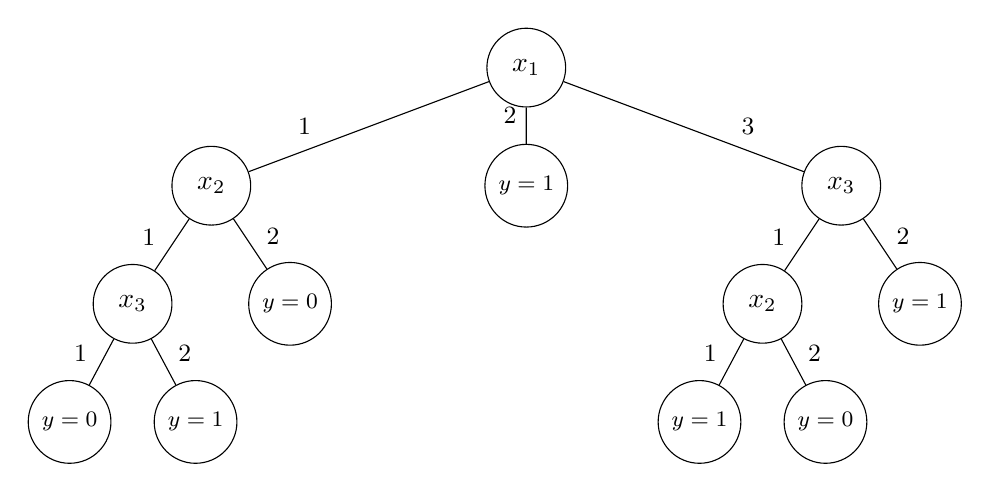
\begin{tikzpicture}[
        level 1/.style={sibling distance=40mm},
        level 2/.style={sibling distance=20mm},
        level 3/.style={sibling distance=16mm},
        split/.style={draw, circle, minimum width=10mm},
        leaf/.style={draw, circle, minimum width=10mm, font=\footnotesize},
        edge from parent/.style={draw, -},
        edge label/.style={font=\small, pos=0.7}
      ]
        \node[split] {$x_1$}
          child {
            node[split] {$x_2$}
            child {
              node[split] {$x_3$}
              child {
                node[leaf] {$y=0$}
                edge from parent node[edge label, above left] {$1$}
              }
              child {
                node[leaf] {$y=1$}
                edge from parent node[edge label, above right] {$2$}
              }
              edge from parent node[edge label, above left] {$1$}
            }
            child {
              node[leaf] {$y=0$}
              edge from parent node[edge label, above right] {$2$}
            }
            edge from parent node[edge label, above left] {$1$}
          }
          child {
            node[leaf] {$y=1$}
            edge from parent node[edge label, above left] {$2$}
          }
          child {
            node[split] {$x_3$}
            child {
              node[split] {$x_2$}
              child {
                node[leaf] {$y=1$}
                edge from parent node[edge label, above left] {$1$}
              }
              child {
                node[leaf] {$y=0$}
                edge from parent node[edge label, above right] {$2$}
              }
              edge from parent node[edge label, above left] {$1$}
            }
            child {
              node[leaf] {$y=1$}
              edge from parent node[edge label, above right] {$2$}
            }
            edge from parent node[edge label, above right] {$3$}
          };
      \end{tikzpicture}
      \caption{An example of a decision tree. Note that the same feature need not be split across all depths (e.g. in depth 1, the leftmost node is split on $x_2$ while the rightmost is split on $x_3$) and the path to a leaf can end early (e.g. there is a node of depth $1$ that is a leaf). }
    \end{figure}
  \end{definition}

  The decision tree tries to take advantage of some nontrivial covariance between $X$ and $Y$ by constructing nested partitions of the dataset $\mathcal{D}$, and within a partition, it predicts the label that comprises the majority. Note that this model is extremely flexible in that we can have different properties of these trees. We will introduce them as we go. 

  \begin{definition}[Binary Decision Tree]
    A \textbf{binary decision tree} only allows the tree to split into two nodes. 
  \end{definition} 

  Note that in density estimation or linear regression, we can derive the risk by first deriving the likelihood of the data, and then taking the negative logarithm of it to get our loss function which allows us to define our risk. In a decision tree, we have a \textit{non-probabilistic} discriminative model, so there is no concept of likelihood. Therefore, we cannot use a pdf to define the loss. Fortunately, we can use the straightforward misclassification risk. 

  \begin{theorem}[Expected and Empirical Risk of Decision Trees]
    Given a classification tree $f$, the misclassification risk over the true data generating distribution $p(x, y)$, along with its empirical risk over a dataset $\mathcal{D} = (x^{(i)}, y^{(i)})_{i=1}^n$, is 
    \begin{align}
      R(f) & = \mathbb{E}_{x, y} \left[ \mathbbm{1} (y \neq f(x))\right] = \int \mathbbm{1} (y \neq f(x)) \, dx \,dy \\ 
      \hat{R}(f) & = \frac{1}{n} \sum_{i=1}^n \mathbbm{1} (y^{(i)} \neq f(x^{(i)}))
    \end{align}
    where $\mathbbm{1}(p)$ is an indicator function that equals $1$ if $p$ is true and $0$ if false. Note that $\hat{R}(f)$ is simply 1 minus the accuracy. 
  \end{theorem} 

  Let's take a look at some examples. The behavior of splitting a node can be different depending on what the covariate is. Given covariate $x_i$, 
  \begin{enumerate}
    \item if $x_i \in \{0, 1\}$, then we can simply split it with left and right children. 
    \item if $x_i \in \{1, \ldots, K\}$, then we can split it across $K$ children. We can also choose a cutoff value for a binary split, e.g. go left if $x_i < t$ and right if $x_i \geq t$. Or, we might choose some subset $S \subset \{1, \ldots, K\}$, where we go left if $x_i \in K$ and right if $x_i \not\in K$. 
    \item if $x_i \in \mathbb{R}$, then we must choose a cutoff value $t$ or partition $\mathbb{R}$ to split. Usually, a cutoff is chosen in practice, since finding a partition leads to a much more difficult problem to learn. 
  \end{enumerate}
  Let's examine this in the following two examples. 

  \begin{example}[Categorical Covariates]
    Consider the following dataset, where we consider a binary classification system with discrete covariates. 

    \begin{table}[H]
      \centering
      {\footnotesize 
      \begin{tabular}{|c|c|c|c|c|c|c|c|c|c|c|}
        \hline
        & OthOptions & Weekend & WaitArea & Plans & Price & Precip & Restaur & Wait & Crowded & Stay? \\
        \hline
        $x_1$ & \textcolor{blue}{Yes} & \textcolor{blue}{No} & \textcolor{blue}{No} & \textcolor{blue}{Yes} & \$\$\$ & \textcolor{blue}{No} & \textcolor{blue}{Mateo} & 0-5 & \textcolor{blue}{some} & Yes \\
        \hline
        $x_2$ & \textcolor{green!50!black}{Yes} & \textcolor{green!50!black}{No} & \textcolor{green!50!black}{No} & \textcolor{green!50!black}{Yes} & \$ & \textcolor{green!50!black}{No} & \textcolor{green!50!black}{Juju} & 16-30 & \textcolor{green!50!black}{full} & No \\
        \hline
        $x_3$ & \textcolor{blue}{No} & \textcolor{blue}{No} & \textcolor{blue}{Yes} & \textcolor{blue}{No} & \$ & \textcolor{blue}{No} & \textcolor{blue}{Pizza} & 0-5 & \textcolor{blue}{some} & Yes \\
        \hline
        $x_4$ & \textcolor{blue}{Yes} & \textcolor{blue}{Yes} & \textcolor{blue}{No} & \textcolor{blue}{Yes} & \$ & \textcolor{blue}{No} & \textcolor{blue}{Juju} & 6-15 & \textcolor{blue}{full} & Yes \\
        \hline
        $x_5$ & \textcolor{green!50!black}{Yes} & \textcolor{green!50!black}{Yes} & \textcolor{green!50!black}{No} & \textcolor{green!50!black}{No} & \$\$\$ & \textcolor{green!50!black}{No} & \textcolor{green!50!black}{Mateo} & 30+ & \textcolor{green!50!black}{full} & No \\
        \hline
        $x_6$ & \textcolor{blue}{No} & \textcolor{blue}{No} & \textcolor{blue}{Yes} & \textcolor{blue}{Yes} & \$\$ & \textcolor{blue}{Yes} & \textcolor{blue}{BlueCorn} & 0-5 & \textcolor{blue}{some} & Yes \\
        \hline
        $x_7$ & \textcolor{green!50!black}{No} & \textcolor{green!50!black}{No} & \textcolor{green!50!black}{Yes} & \textcolor{green!50!black}{No} & \$ & \textcolor{green!50!black}{Yes} & \textcolor{green!50!black}{Pizza} & 0-5 & \textcolor{green!50!black}{none} & No \\
        \hline
        $x_8$ & \textcolor{blue}{No} & \textcolor{blue}{No} & \textcolor{blue}{No} & \textcolor{blue}{Yes} & \$\$ & \textcolor{blue}{Yes} & \textcolor{blue}{Juju} & 0-5 & \textcolor{blue}{some} & Yes \\
        \hline
        $x_9$ & \textcolor{green!50!black}{No} & \textcolor{green!50!black}{Yes} & \textcolor{green!50!black}{Yes} & \textcolor{green!50!black}{No} & \$ & \textcolor{green!50!black}{Yes} & \textcolor{green!50!black}{Pizza} & 30+ & \textcolor{green!50!black}{full} & No \\
        \hline
        $x_{10}$ & \textcolor{green!50!black}{Yes} & \textcolor{green!50!black}{Yes} & \textcolor{green!50!black}{Yes} & \textcolor{green!50!black}{Yes} & \$\$\$ & \textcolor{green!50!black}{No} & \textcolor{green!50!black}{BlueCorn} & 6-15 & \textcolor{green!50!black}{full} & No \\
        \hline
        $x_{11}$ & \textcolor{green!50!black}{No} & \textcolor{green!50!black}{No} & \textcolor{green!50!black}{No} & \textcolor{green!50!black}{No} & \$ & \textcolor{green!50!black}{No} & \textcolor{green!50!black}{Juju} & 0-5 & \textcolor{green!50!black}{none} & No \\
        \hline
        $x_{12}$ & \textcolor{blue}{Yes} & \textcolor{blue}{Yes} & \textcolor{blue}{Yes} & \textcolor{blue}{Yes} & \$ & \textcolor{blue}{No} & \textcolor{blue}{Pizza} & 16-30 & \textcolor{blue}{full} & Yes \\
        \hline
      \end{tabular}
      }
      \caption{Dataset of whether to go to a restaurant for a date depending on certain factors. }
      \label{tab:restaurant}
    \end{table}

    This is a binary classification problem, and we can count that there are $6$ positives and $6$ negative labels. Let's evaluate the accuracy of some example trees. 

    \begin{figure}[H]
      \centering
      \begin{subfigure}[b]{0.48\textwidth}
        \centering
        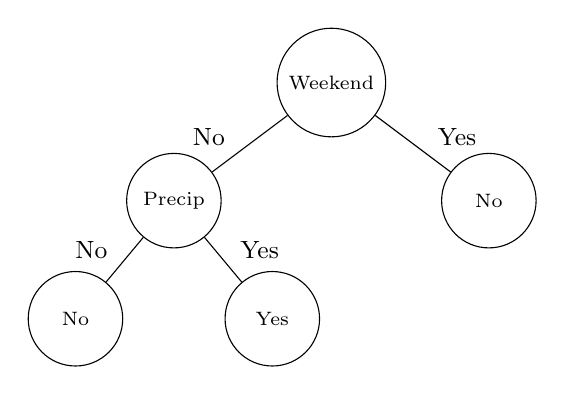
\begin{tikzpicture}[
          level 1/.style={sibling distance=40mm},
          level 2/.style={sibling distance=25mm},
          split/.style={draw, circle, minimum width=12mm, font=\scriptsize},
          leaf/.style={draw, circle, minimum width=12mm, font=\scriptsize},
          edge from parent/.style={draw, -},
          edge label/.style={font=\small, pos=0.7}
        ]
          \node[split] {Weekend}
            child {
              node[split] {Precip}
              child {
                node[leaf] {No}
                edge from parent node[edge label, above left] {No}
              }
              child {
                node[leaf] {Yes}
                edge from parent node[edge label, above right] {Yes}
              }
              edge from parent node[edge label, above left] {No}
            }
            child {
              node[leaf] {No}
              edge from parent node[edge label, above right] {Yes}
            };
        \end{tikzpicture}
        \caption{The accuracy of this tree is 7 out of 12. }
      \end{subfigure}
      \hfill 
      \begin{subfigure}[b]{0.48\textwidth}
        \centering
        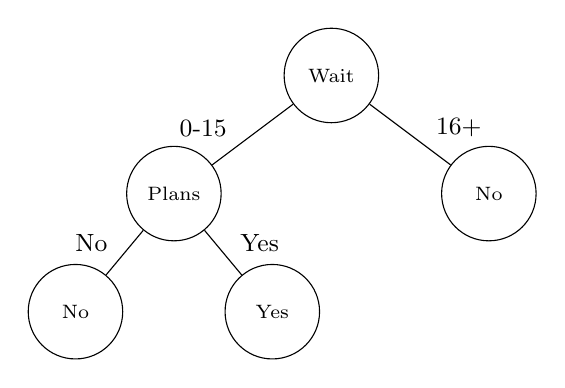
\begin{tikzpicture}[
          level 1/.style={sibling distance=40mm},
          level 2/.style={sibling distance=25mm},
          split/.style={draw, circle, minimum width=12mm, font=\scriptsize},
          leaf/.style={draw, circle, minimum width=12mm, font=\scriptsize},
          edge from parent/.style={draw, -},
          edge label/.style={font=\small, pos=0.7}
        ]
          \node[split] {Wait}
            child {
              node[split] {Plans}
              child {
                node[leaf] {No}
                edge from parent node[edge label, above left] {No}
              }
              child {
                node[leaf] {Yes}
                edge from parent node[edge label, above right] {Yes}
              }
              edge from parent node[edge label, above left] {0-15}
            }
            child {
              node[leaf] {No}
              edge from parent node[edge label, above right] {16+}
            };
        \end{tikzpicture}
        \caption{The accuracy of this tree is 9 out of 12.}
      \end{subfigure}
      \caption{Even though the trees have the same structure, the features that they split on has high impact on the accuracy.}
    \end{figure}
  \end{example}

  \begin{example}[Continuous Covariates]
    Now let's take a look at a dataset with continuous covariates. 

    \begin{table}[H]
      \centering
      {\footnotesize 
      \begin{tabular}{|c|c|c|c|c|c|c|c|c|c|c|}
        \hline
        & Size & Age & Bedrooms & Distance & Crime & Income & Schools & Garage & Lot & Expensive? \\
        \hline
        $x_1$ & \textcolor{blue}{2400} & \textcolor{blue}{8} & \textcolor{blue}{3.0} & \textcolor{blue}{2.1} & \textcolor{blue}{1.2} & \textcolor{blue}{85} & \textcolor{blue}{8.7} & \textcolor{blue}{2.0} & \textcolor{blue}{0.31} & Yes \\
        \hline
        $x_2$ & \textcolor{green!50!black}{1200} & \textcolor{green!50!black}{45} & \textcolor{green!50!black}{2.0} & \textcolor{green!50!black}{8.7} & \textcolor{green!50!black}{4.8} & \textcolor{green!50!black}{42} & \textcolor{green!50!black}{5.2} & \textcolor{green!50!black}{1.0} & \textcolor{green!50!black}{0.18} & No \\
        \hline
        $x_3$ & \textcolor{blue}{3100} & \textcolor{blue}{12} & \textcolor{blue}{4.0} & \textcolor{blue}{1.4} & \textcolor{blue}{0.9} & \textcolor{blue}{92} & \textcolor{blue}{9.1} & \textcolor{blue}{2.5} & \textcolor{blue}{0.45} & Yes \\
        \hline
        $x_4$ & \textcolor{blue}{2800} & \textcolor{blue}{6} & \textcolor{blue}{3.5} & \textcolor{blue}{3.2} & \textcolor{blue}{2.1} & \textcolor{blue}{78} & \textcolor{blue}{8.3} & \textcolor{blue}{2.0} & \textcolor{blue}{0.28} & Yes \\
        \hline
        $x_5$ & \textcolor{green!50!black}{950} & \textcolor{green!50!black}{62} & \textcolor{green!50!black}{1.5} & \textcolor{green!50!black}{12.3} & \textcolor{green!50!black}{6.7} & \textcolor{green!50!black}{35} & \textcolor{green!50!black}{4.1} & \textcolor{green!50!black}{0.5} & \textcolor{green!50!black}{0.12} & No \\
        \hline
        $x_6$ & \textcolor{blue}{2650} & \textcolor{blue}{15} & \textcolor{blue}{3.0} & \textcolor{blue}{2.8} & \textcolor{blue}{1.7} & \textcolor{blue}{68} & \textcolor{blue}{7.9} & \textcolor{blue}{2.0} & \textcolor{blue}{0.35} & Yes \\
        \hline
        $x_7$ & \textcolor{green!50!black}{1450} & \textcolor{green!50!black}{38} & \textcolor{green!50!black}{2.5} & \textcolor{green!50!black}{7.1} & \textcolor{green!50!black}{5.2} & \textcolor{green!50!black}{48} & \textcolor{green!50!black}{6.0} & \textcolor{green!50!black}{1.0} & \textcolor{green!50!black}{0.22} & No \\
        \hline
        $x_8$ & \textcolor{blue}{2200} & \textcolor{blue}{22} & \textcolor{blue}{3.0} & \textcolor{blue}{4.5} & \textcolor{blue}{2.8} & \textcolor{blue}{71} & \textcolor{blue}{7.4} & \textcolor{blue}{1.5} & \textcolor{blue}{0.26} & Yes \\
        \hline
        $x_9$ & \textcolor{green!50!black}{1100} & \textcolor{green!50!black}{55} & \textcolor{green!50!black}{2.0} & \textcolor{green!50!black}{9.8} & \textcolor{green!50!black}{5.9} & \textcolor{green!50!black}{39} & \textcolor{green!50!black}{4.8} & \textcolor{green!50!black}{1.0} & \textcolor{green!50!black}{0.15} & No \\
        \hline
        $x_{10}$ & \textcolor{green!50!black}{1800} & \textcolor{green!50!black}{28} & \textcolor{green!50!black}{2.5} & \textcolor{green!50!black}{6.2} & \textcolor{green!50!black}{3.4} & \textcolor{green!50!black}{55} & \textcolor{green!50!black}{6.7} & \textcolor{green!50!black}{1.5} & \textcolor{green!50!black}{0.20} & No \\
        \hline
        $x_{11}$ & \textcolor{green!50!black}{1350} & \textcolor{green!50!black}{41} & \textcolor{green!50!black}{2.0} & \textcolor{green!50!black}{8.9} & \textcolor{green!50!black}{4.6} & \textcolor{green!50!black}{44} & \textcolor{green!50!black}{5.5} & \textcolor{green!50!black}{1.0} & \textcolor{green!50!black}{0.19} & No \\
        \hline
        $x_{12}$ & \textcolor{blue}{2900} & \textcolor{blue}{10} & \textcolor{blue}{4.0} & \textcolor{blue}{1.8} & \textcolor{blue}{1.4} & \textcolor{blue}{88} & \textcolor{blue}{8.9} & \textcolor{blue}{2.5} & \textcolor{blue}{0.42} & Yes \\
        \hline
      \end{tabular}
      }
      \caption{Dataset for predicting whether a house is expensive (\$500K+) based on continuous features. Size (sq ft), Age (years), Bedrooms (count), Distance (miles to downtown), Crime (incidents per 1000), Income (neighborhood median in \$1000s), Schools (rating 1-10), Garage (spaces), Lot (acres).}
      \label{tab:housing}
    \end{table}

    \begin{figure}[H]
      \centering
      \begin{subfigure}[b]{0.48\textwidth}
        \centering
        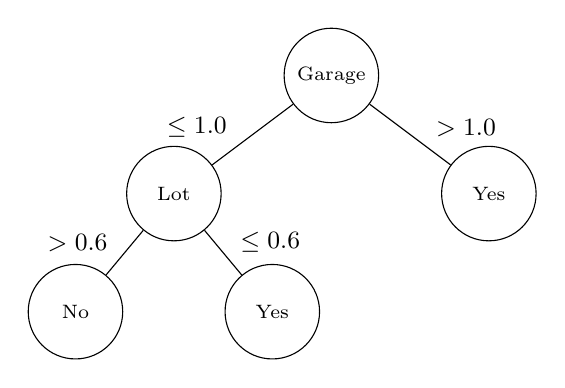
\begin{tikzpicture}[
          level 1/.style={sibling distance=40mm},
          level 2/.style={sibling distance=25mm},
          split/.style={draw, circle, minimum width=12mm, font=\scriptsize},
          leaf/.style={draw, circle, minimum width=12mm, font=\scriptsize},
          edge from parent/.style={draw, -},
          edge label/.style={font=\small, pos=0.7}
        ]
          \node[split] {Garage}
            child {
              node[split] {Lot}
              child {
                node[leaf] {No}
                edge from parent node[edge label, above left] {$> 0.6$}
              }
              child {
                node[leaf] {Yes}
                edge from parent node[edge label, above right] {$\leq 0.6$}
              }
              edge from parent node[edge label, above left] {$\leq 1.0$}
            }
            child {
              node[leaf] {Yes}
              edge from parent node[edge label, above right] {$> 1.0$}
            };
        \end{tikzpicture}
        \caption{The accuracy of this tree is 7 out of 12.}
      \end{subfigure}
      \hfill 
      \begin{subfigure}[b]{0.48\textwidth}
        \centering
        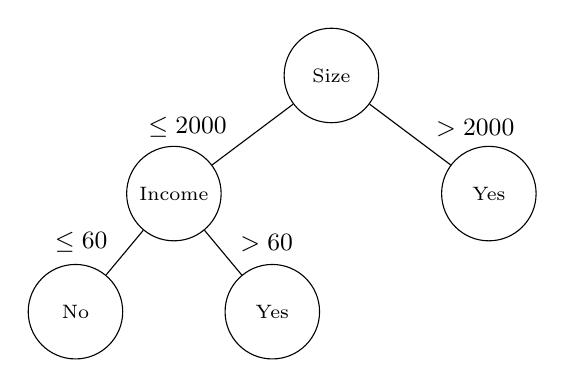
\begin{tikzpicture}[
          level 1/.style={sibling distance=40mm},
          level 2/.style={sibling distance=25mm},
          split/.style={draw, circle, minimum width=12mm, font=\scriptsize},
          leaf/.style={draw, circle, minimum width=12mm, font=\scriptsize},
          edge from parent/.style={draw, -},
          edge label/.style={font=\small, pos=0.7}
        ]
          \node[split] {Size}
            child {
              node[split] {Income}
              child {
                node[leaf] {No}
                edge from parent node[edge label, above left] {$\leq 60$}
              }
              child {
                node[leaf] {Yes}
                edge from parent node[edge label, above right] {$> 60$}
              }
              edge from parent node[edge label, above left] {$\leq 2000$}
            }
            child {
              node[leaf] {Yes}
              edge from parent node[edge label, above right] {$> 2000$}
            };
        \end{tikzpicture}
        \caption{The accuracy of this tree is 12 out of 12.}
      \end{subfigure}
      \caption{}
    \end{figure}
  \end{example}

  This is all nice in theory, but how are we supposed to optimize this in practice? First, the misclassification loss is not differentiable---and even worse---the gradient is $0$ almost everywhere! This isn't as bad as it seems, since we can introduce a surrogate loss function and optimize that. The big problem is that $f$ is not parameteric, so we can't even gradients at all (with respect to what parameter?)! One solution is to try and create a very specific tree model---making it parameteric---and then using a surrogate loss to learn. In fact this done in practice, but for now let's keep things simple and hold off on this problem until later. 

\subsection{Regression Trees}

  Regression trees behave similarly to classification trees, but now the outputs are meant to be continuous. Clearly, a tree having a discrete set of leaf nodes cannot fit a continuum, but we can try to fit it with step functions. 

  \begin{definition}[Regression Tree]
    A \textbf{regression tree} is a nonparameteric discriminative model $f: X \to \mathbb{R}$, that uses a tree representing a set of decisions on an input $x$ to predict a value $y$. 

    \begin{figure}[H]
      \centering 
      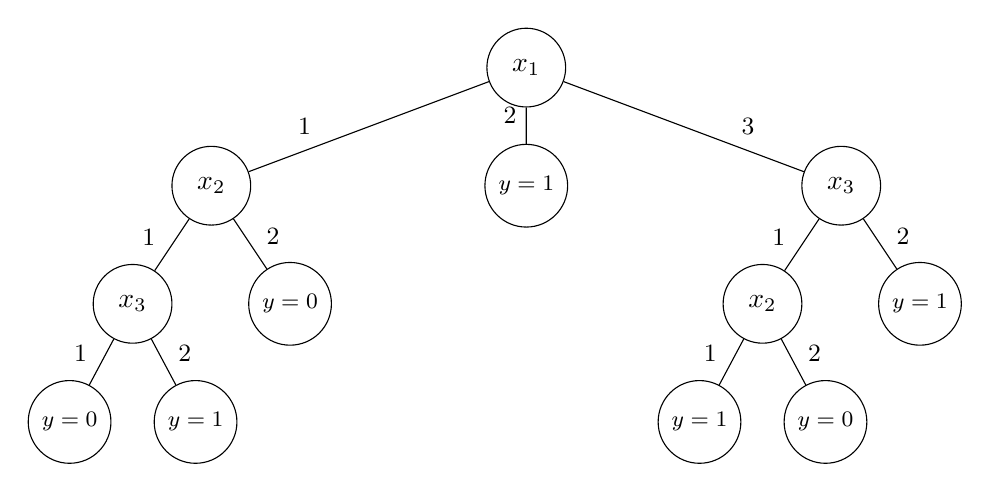
\begin{tikzpicture}[
        level 1/.style={sibling distance=40mm},
        level 2/.style={sibling distance=20mm},
        level 3/.style={sibling distance=16mm},
        split/.style={draw, circle, minimum width=10mm},
        leaf/.style={draw, circle, minimum width=10mm, font=\footnotesize},
        edge from parent/.style={draw, -},
        edge label/.style={font=\small, pos=0.7}
      ]
        \node[split] {$x_1$}
          child {
            node[split] {$x_2$}
            child {
              node[split] {$x_3$}
              child {
                node[leaf] {$y=0$}
                edge from parent node[edge label, above left] {$1$}
              }
              child {
                node[leaf] {$y=1$}
                edge from parent node[edge label, above right] {$2$}
              }
              edge from parent node[edge label, above left] {$1$}
            }
            child {
              node[leaf] {$y=0$}
              edge from parent node[edge label, above right] {$2$}
            }
            edge from parent node[edge label, above left] {$1$}
          }
          child {
            node[leaf] {$y=1$}
            edge from parent node[edge label, above left] {$2$}
          }
          child {
            node[split] {$x_3$}
            child {
              node[split] {$x_2$}
              child {
                node[leaf] {$y=1$}
                edge from parent node[edge label, above left] {$1$}
              }
              child {
                node[leaf] {$y=0$}
                edge from parent node[edge label, above right] {$2$}
              }
              edge from parent node[edge label, above left] {$1$}
            }
            child {
              node[leaf] {$y=1$}
              edge from parent node[edge label, above right] {$2$}
            }
            edge from parent node[edge label, above right] {$3$}
          };
      \end{tikzpicture}
      \caption{An example of a decision tree. Note that the same feature need not be split across all depths (e.g. in depth 1, the leftmost node is split on $x_2$ while the rightmost is split on $x_3$) and the path to a leaf can end early (e.g. there is a node of depth $1$ that is a leaf). }
    \end{figure}
  \end{definition}

  \begin{example}[Regression on Categorical Covariates]
    \begin{table}[H]
      \centering
      {\footnotesize 
      \begin{tabular}{|c|c|c|c|c|c|c|c|c|c|c|}
        \hline
        & OthOptions & Weekend & WaitArea & Plans & Price & Precip & Restaur & Wait & Crowded & Tip\% \\
        \hline
        $x_1$ & \textcolor{blue}{Yes} & \textcolor{blue}{No} & \textcolor{blue}{No} & \textcolor{blue}{Yes} & \$\$\$ & \textcolor{blue}{No} & \textcolor{blue}{Mateo} & 0-5 & \textcolor{blue}{some} & 22\% \\
        \hline
        $x_2$ & \textcolor{green!50!black}{Yes} & \textcolor{green!50!black}{No} & \textcolor{green!50!black}{No} & \textcolor{green!50!black}{Yes} & \$ & \textcolor{green!50!black}{No} & \textcolor{green!50!black}{Juju} & 16-30 & \textcolor{green!50!black}{full} & 12\% \\
        \hline
        $x_3$ & \textcolor{blue}{No} & \textcolor{blue}{No} & \textcolor{blue}{Yes} & \textcolor{blue}{No} & \$ & \textcolor{blue}{No} & \textcolor{blue}{Pizza} & 0-5 & \textcolor{blue}{some} & 18\% \\
        \hline
        $x_4$ & \textcolor{blue}{Yes} & \textcolor{blue}{Yes} & \textcolor{blue}{No} & \textcolor{blue}{Yes} & \$ & \textcolor{blue}{No} & \textcolor{blue}{Juju} & 6-15 & \textcolor{blue}{full} & 20\% \\
        \hline
        $x_5$ & \textcolor{green!50!black}{Yes} & \textcolor{green!50!black}{Yes} & \textcolor{green!50!black}{No} & \textcolor{green!50!black}{No} & \$\$\$ & \textcolor{green!50!black}{No} & \textcolor{green!50!black}{Mateo} & 30+ & \textcolor{green!50!black}{full} & 8\% \\
        \hline
        $x_6$ & \textcolor{blue}{No} & \textcolor{blue}{No} & \textcolor{blue}{Yes} & \textcolor{blue}{Yes} & \$\$ & \textcolor{blue}{Yes} & \textcolor{blue}{BlueCorn} & 0-5 & \textcolor{blue}{some} & 25\% \\
        \hline
        $x_7$ & \textcolor{green!50!black}{No} & \textcolor{green!50!black}{No} & \textcolor{green!50!black}{Yes} & \textcolor{green!50!black}{No} & \$ & \textcolor{green!50!black}{Yes} & \textcolor{green!50!black}{Pizza} & 0-5 & \textcolor{green!50!black}{none} & 15\% \\
        \hline
        $x_8$ & \textcolor{blue}{No} & \textcolor{blue}{No} & \textcolor{blue}{No} & \textcolor{blue}{Yes} & \$\$ & \textcolor{blue}{Yes} & \textcolor{blue}{Juju} & 0-5 & \textcolor{blue}{some} & 23\% \\
        \hline
        $x_9$ & \textcolor{green!50!black}{No} & \textcolor{green!50!black}{Yes} & \textcolor{green!50!black}{Yes} & \textcolor{green!50!black}{No} & \$ & \textcolor{green!50!black}{Yes} & \textcolor{green!50!black}{Pizza} & 30+ & \textcolor{green!50!black}{full} & 10\% \\
        \hline
        $x_{10}$ & \textcolor{green!50!black}{Yes} & \textcolor{green!50!black}{Yes} & \textcolor{green!50!black}{Yes} & \textcolor{green!50!black}{Yes} & \$\$\$ & \textcolor{green!50!black}{No} & \textcolor{green!50!black}{BlueCorn} & 6-15 & \textcolor{green!50!black}{full} & 14\% \\
        \hline
        $x_{11}$ & \textcolor{green!50!black}{No} & \textcolor{green!50!black}{No} & \textcolor{green!50!black}{No} & \textcolor{green!50!black}{No} & \$ & \textcolor{green!50!black}{No} & \textcolor{green!50!black}{Juju} & 0-5 & \textcolor{green!50!black}{none} & 16\% \\
        \hline
        $x_{12}$ & \textcolor{blue}{Yes} & \textcolor{blue}{Yes} & \textcolor{blue}{Yes} & \textcolor{blue}{Yes} & \$ & \textcolor{blue}{No} & \textcolor{blue}{Pizza} & 16-30 & \textcolor{blue}{full} & 19\% \\
        \hline
      \end{tabular}
      }
      \caption{Dataset for predicting tip percentage based on restaurant dining factors.}
      \label{tab:restaurant_tips}
    \end{table} 

    \begin{figure}[H]
      \centering
      \begin{subfigure}[b]{0.48\textwidth}
        \centering
        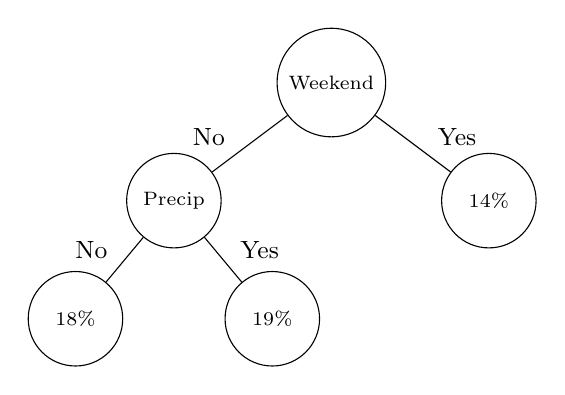
\begin{tikzpicture}[
          level 1/.style={sibling distance=40mm},
          level 2/.style={sibling distance=25mm},
          split/.style={draw, circle, minimum width=12mm, font=\scriptsize},
          leaf/.style={draw, circle, minimum width=12mm, font=\scriptsize},
          edge from parent/.style={draw, -},
          edge label/.style={font=\small, pos=0.7}
        ]
          \node[split] {Weekend}
            child {
              node[split] {Precip}
              child {
                node[leaf] {18\%}
                edge from parent node[edge label, above left] {No}
              }
              child {
                node[leaf] {19\%}
                edge from parent node[edge label, above right] {Yes}
              }
              edge from parent node[edge label, above left] {No}
            }
            child {
              node[leaf] {14\%}
              edge from parent node[edge label, above right] {Yes}
            };
        \end{tikzpicture}
        \caption{Bad tree splits on Weekend first, then Precip. Mean Absolute Error: 4.2\%}
      \end{subfigure}
      \hfill 
      \begin{subfigure}[b]{0.48\textwidth}
        \centering
        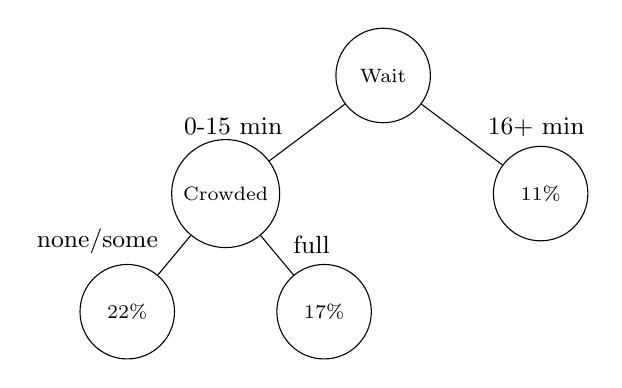
\begin{tikzpicture}[
          level 1/.style={sibling distance=40mm},
          level 2/.style={sibling distance=25mm},
          split/.style={draw, circle, minimum width=12mm, font=\scriptsize},
          leaf/.style={draw, circle, minimum width=12mm, font=\scriptsize},
          edge from parent/.style={draw, -},
          edge label/.style={font=\small, pos=0.7}
        ]
          \node[split] {Wait}
            child {
              node[split] {Crowded}
              child {
                node[leaf] {22\%}
                edge from parent node[edge label, above left] {none/some}
              }
              child {
                node[leaf] {17\%}
                edge from parent node[edge label, above right] {full}
              }
              edge from parent node[edge label, above left] {0-15 min}
            }
            child {
              node[leaf] {11\%}
              edge from parent node[edge label, above right] {16+ min}
            };
        \end{tikzpicture}
        \caption{Good tree splits on Wait first, then Crowded. Mean Absolute Error: 2.1\%}
      \end{subfigure}
      \caption{Comparison of regression trees for predicting tip percentage. The good tree using Wait time and Crowded level achieves much better prediction accuracy than the bad tree using Weekend and Precipitation.}
    \end{figure}
  \end{example}

  \begin{example}[Regression on Continuous Covariates]
    \begin{table}[H]
      \centering
      {\footnotesize 
      \begin{tabular}{|c|c|c|c|c|c|c|c|c|c|c|}
        \hline
        & Size & Age & Bedrooms & Distance & Crime & Income & Schools & Garage & Lot & Price \\
        \hline
        $x_1$ & \textcolor{blue}{2400} & \textcolor{blue}{8} & \textcolor{blue}{3.0} & \textcolor{blue}{2.1} & \textcolor{blue}{1.2} & \textcolor{blue}{85} & \textcolor{blue}{8.7} & \textcolor{blue}{2.0} & \textcolor{blue}{0.31} & \$645K \\
        \hline
        $x_2$ & \textcolor{green!50!black}{1200} & \textcolor{green!50!black}{45} & \textcolor{green!50!black}{2.0} & \textcolor{green!50!black}{8.7} & \textcolor{green!50!black}{4.8} & \textcolor{green!50!black}{42} & \textcolor{green!50!black}{5.2} & \textcolor{green!50!black}{1.0} & \textcolor{green!50!black}{0.18} & \$285K \\
        \hline
        $x_3$ & \textcolor{blue}{3100} & \textcolor{blue}{12} & \textcolor{blue}{4.0} & \textcolor{blue}{1.4} & \textcolor{blue}{0.9} & \textcolor{blue}{92} & \textcolor{blue}{9.1} & \textcolor{blue}{2.5} & \textcolor{blue}{0.45} & \$825K \\
        \hline
        $x_4$ & \textcolor{blue}{2800} & \textcolor{blue}{6} & \textcolor{blue}{3.5} & \textcolor{blue}{3.2} & \textcolor{blue}{2.1} & \textcolor{blue}{78} & \textcolor{blue}{8.3} & \textcolor{blue}{2.0} & \textcolor{blue}{0.28} & \$710K \\
        \hline
        $x_5$ & \textcolor{green!50!black}{950} & \textcolor{green!50!black}{62} & \textcolor{green!50!black}{1.5} & \textcolor{green!50!black}{12.3} & \textcolor{green!50!black}{6.7} & \textcolor{green!50!black}{35} & \textcolor{green!50!black}{4.1} & \textcolor{green!50!black}{0.5} & \textcolor{green!50!black}{0.12} & \$195K \\
        \hline
        $x_6$ & \textcolor{blue}{2650} & \textcolor{blue}{15} & \textcolor{blue}{3.0} & \textcolor{blue}{2.8} & \textcolor{blue}{1.7} & \textcolor{blue}{68} & \textcolor{blue}{7.9} & \textcolor{blue}{2.0} & \textcolor{blue}{0.35} & \$580K \\
        \hline
        $x_7$ & \textcolor{green!50!black}{1450} & \textcolor{green!50!black}{38} & \textcolor{green!50!black}{2.5} & \textcolor{green!50!black}{7.1} & \textcolor{green!50!black}{5.2} & \textcolor{green!50!black}{48} & \textcolor{green!50!black}{6.0} & \textcolor{green!50!black}{1.0} & \textcolor{green!50!black}{0.22} & \$325K \\
        \hline
        $x_8$ & \textcolor{blue}{2200} & \textcolor{blue}{22} & \textcolor{blue}{3.0} & \textcolor{blue}{4.5} & \textcolor{blue}{2.8} & \textcolor{blue}{71} & \textcolor{blue}{7.4} & \textcolor{blue}{1.5} & \textcolor{blue}{0.26} & \$515K \\
        \hline
        $x_9$ & \textcolor{green!50!black}{1100} & \textcolor{green!50!black}{55} & \textcolor{green!50!black}{2.0} & \textcolor{green!50!black}{9.8} & \textcolor{green!50!black}{5.9} & \textcolor{green!50!black}{39} & \textcolor{green!50!black}{4.8} & \textcolor{green!50!black}{1.0} & \textcolor{green!50!black}{0.15} & \$240K \\
        \hline
        $x_{10}$ & \textcolor{green!50!black}{1800} & \textcolor{green!50!black}{28} & \textcolor{green!50!black}{2.5} & \textcolor{green!50!black}{6.2} & \textcolor{green!50!black}{3.4} & \textcolor{green!50!black}{55} & \textcolor{green!50!black}{6.7} & \textcolor{green!50!black}{1.5} & \textcolor{green!50!black}{0.20} & \$385K \\
        \hline
        $x_{11}$ & \textcolor{green!50!black}{1350} & \textcolor{green!50!black}{41} & \textcolor{green!50!black}{2.0} & \textcolor{green!50!black}{8.9} & \textcolor{green!50!black}{4.6} & \textcolor{green!50!black}{44} & \textcolor{green!50!black}{5.5} & \textcolor{green!50!black}{1.0} & \textcolor{green!50!black}{0.19} & \$295K \\
        \hline
        $x_{12}$ & \textcolor{blue}{2900} & \textcolor{blue}{10} & \textcolor{blue}{4.0} & \textcolor{blue}{1.8} & \textcolor{blue}{1.4} & \textcolor{blue}{88} & \textcolor{blue}{8.9} & \textcolor{blue}{2.5} & \textcolor{blue}{0.42} & \$780K \\
        \hline
      \end{tabular}
      }
      \caption{Dataset for predicting house prices based on continuous features. Size (sq ft), Age (years), Bedrooms (count), Distance (miles to downtown), Crime (incidents per 1000), Income (neighborhood median in \$1000s), Schools (rating 1-10), Garage (spaces), Lot (acres).}
      \label{tab:housing_prices}
    \end{table} 

    \begin{figure}[H]
      \centering
      \begin{subfigure}[b]{0.48\textwidth}
        \centering
        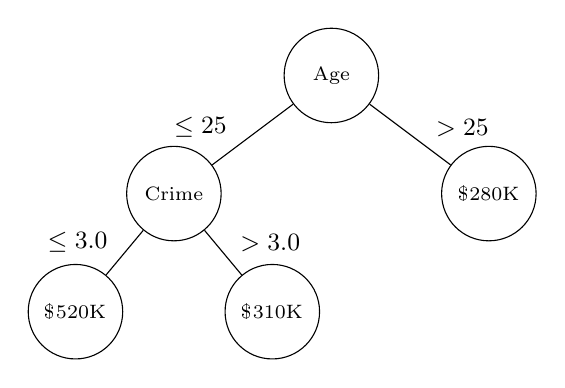
\begin{tikzpicture}[
          level 1/.style={sibling distance=40mm},
          level 2/.style={sibling distance=25mm},
          split/.style={draw, circle, minimum width=12mm, font=\scriptsize},
          leaf/.style={draw, circle, minimum width=12mm, font=\scriptsize},
          edge from parent/.style={draw, -},
          edge label/.style={font=\small, pos=0.7}
        ]
          \node[split] {Age}
            child {
              node[split] {Crime}
              child {
                node[leaf] {\$520K}
                edge from parent node[edge label, above left] {$\leq 3.0$}
              }
              child {
                node[leaf] {\$310K}
                edge from parent node[edge label, above right] {$> 3.0$}
              }
              edge from parent node[edge label, above left] {$\leq 25$}
            }
            child {
              node[leaf] {\$280K}
              edge from parent node[edge label, above right] {$> 25$}
            };
        \end{tikzpicture}
        \caption{Bad tree splits on Age first, then Crime. Mean Absolute Error: \$145K}
      \end{subfigure}
      \hfill 
      \begin{subfigure}[b]{0.48\textwidth}
        \centering
        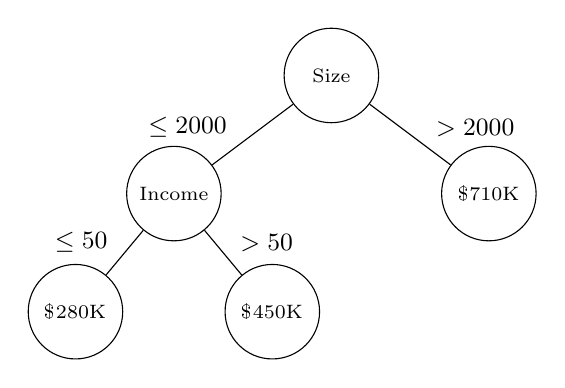
\begin{tikzpicture}[
          level 1/.style={sibling distance=40mm},
          level 2/.style={sibling distance=25mm},
          split/.style={draw, circle, minimum width=12mm, font=\scriptsize},
          leaf/.style={draw, circle, minimum width=12mm, font=\scriptsize},
          edge from parent/.style={draw, -},
          edge label/.style={font=\small, pos=0.7}
        ]
          \node[split] {Size}
            child {
              node[split] {Income}
              child {
                node[leaf] {\$280K}
                edge from parent node[edge label, above left] {$\leq 50$}
              }
              child {
                node[leaf] {\$450K}
                edge from parent node[edge label, above right] {$> 50$}
              }
              edge from parent node[edge label, above left] {$\leq 2000$}
            }
            child {
              node[leaf] {\$710K}
              edge from parent node[edge label, above right] {$> 2000$}
            };
        \end{tikzpicture}
        \caption{Good tree splits on Size first, then Income. Mean Absolute Error: \$65K}
      \end{subfigure}
      \caption{Even though the trees have the same structure, the features they split on have high impact on prediction accuracy. The good tree uses more predictive features (Size and Income) resulting in much lower prediction error.}
    \end{figure}
  \end{example}

  The next question to ask is how we choose the threshold. Essentially, given a set of points $p_1 < p_2 < \ldots < p_n$, where we want to divide $p_1, \ldots, p_k$ and $p_{k+1} < \ldots < p_n$, which value of $t \in (p_k, p_{k+1})$ should we choose? This depends on the optimization algorithm we are using, but one would be to just choose the midpoint. Another would be to take a weighted average of the points. 

\subsection{Model Space} 

  The fact that trees are nonparameteric means that we have extreme flexibility in designing our tree. However, this comes with the big risk of having too big of a model space to optimize over. This overcomplexity is one of the big challenges in trees. 

  For example, suppose that there are $d$ covariates (independent variables, features) $x_1, \ldots, x_d$ all binary valued. We can design a decision tree that splits on $x_1$, then on $x_2$, then on $x_1$, then on $x_2$, and so on. This becomes unbounded and our model space a discrete infinite space, which is a bad combination since we don't have gradients to optimize over a continuum. We can try and handle this in two ways. 

  \begin{example}[Splitting on Same Variable Multiple Times]
    Splitting on covariate $x_1$ infinitely many times seems pretty unrealistic, so we should limit it in some way. 
    \begin{enumerate}
      \item \textit{Covariate can be split a maximum of once for each path from root to leaf}. This is a common assumption for simple problems but may lead to insufficient complexity. In some cases, we would like to look at feature $x_i$, then filter it through $x_j$, and then look at $x_i$ again.
      \item \textit{Covariate can be split maximum of $k$ times}. This can be a practical assumption, but if $k$ is set too high, our model space may be too complex. 
    \end{enumerate}
  \end{example}

  \begin{example}[Depth of Tree]
    Another similar---but distinct---way of restricting the model space is to limit the depth (defined as the maximum length of a path from root to any leaf) of the tree. 
  \end{example} 
  
  Now that we have some restrictions, let's try to analyze the model space.   

  \begin{lemma}[Set of All Full Trees of a Certain Depth]
    Let $x_1, \ldots, x_d$ be binary categorical variables. Let $\mathcal{F}$ be the set of all \textit{perfect}\footnote{Every nonleaf node has a two children, and all leaves are on the same depth} binary decision trees of depth $k$ on a classification problem of $C$ classes. Then, 
    \begin{equation}
      |\mathcal{F}| = d^{2^{k-1}} \cdot C^{2^{k}}
    \end{equation}
  \end{lemma}
  \begin{proof}
    For depth $k$, there are a total of $2^k$ leaf nodes and $2^{k-1}$ internal nodes. Each of the internal nodes can split on any of the $d$ covariates, and the $2^k$ leaf nodes can take any of the $C$ classes. 
  \end{proof}

  This lemma should scare you in that the model complexity is super-exponential with respect to $k$. It would be much higher if we considered non-perfect classification trees and/or non-binary covariates. 

  \begin{example}[Max Subnodes per Split]
    If we did have a multiclass covariate $x_i$ taking values in a set $S$, creating a general partition is equivalent to identifying an ordered partition 
    \begin{equation}
      S = \bigsqcup_{j=1}^m S^\prime_j, \qquad S^\prime_j \neq \emptyset
    \end{equation} 
    where if $x_i \in S^\prime_j$, then it would get routed to the $j$th child. If a node must have $m$ children, then we must consider all $m$-partitions of $S$, which is super-exponential. This becomes worse if a node can have \textit{up to} $m$ children. This is clearly too complex, so we could think of limiting the number of children so that $m = 2$, i.e. we are only allowed to do binary splits. Note that even with this, there are still $2^{|S|} - 2$ ways to split.\footnote{We can choose any arbitrary subset $R \subset S$, which gives us the partition $R \sqcup R^c = S$. $R$ gets routed to the right node and $R^c$ gets routed to the left. We subtract $2$ to make sure that $R, R^C \neq \emptyset$.}
  \end{example}

  This is not all. It is well known that different trees are \textit{functionally} the same. 

  \begin{example}[Model Equivalence]
    The trees below are functionally equal the function 
    \begin{equation}
      f(x) = \begin{cases} 
        0 & \text{ if } (A, B) = (0, 0) \\
        1 & \text{ if } (A, B) = (0, 1) \\
        1 & \text{ if } (A, B) = (1, 0) \\
        0 & \text{ if } (A, B) = (1, 1)
      \end{cases}
    \end{equation}

    \begin{figure}[H]
      \centering
      \begin{subfigure}[b]{0.48\textwidth}
        \centering
        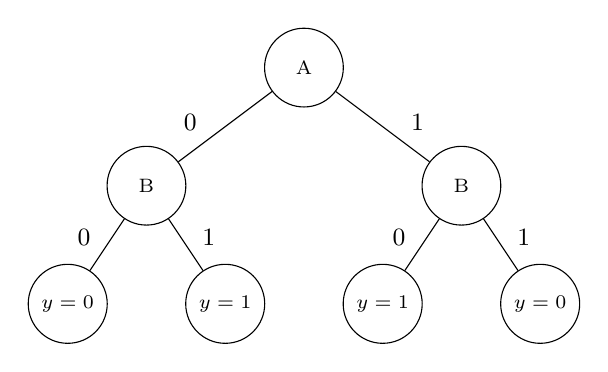
\begin{tikzpicture}[
          level 1/.style={sibling distance=40mm},
          level 2/.style={sibling distance=20mm},
          split/.style={draw, circle, minimum width=10mm, font=\scriptsize},
          leaf/.style={draw, circle, minimum width=10mm, font=\scriptsize},
          edge from parent/.style={draw, -},
          edge label/.style={font=\small, pos=0.7}
        ]
          \node[split] {A}
            child {
              node[split] {B}
              child {
                node[leaf] {$y=0$}
                edge from parent node[edge label, above left] {0}
              }
              child {
                node[leaf] {$y=1$}
                edge from parent node[edge label, above right] {1}
              }
              edge from parent node[edge label, above left] {0}
            }
            child {
              node[split] {B}
              child {
                node[leaf] {$y=1$}
                edge from parent node[edge label, above left] {0}
              }
              child {
                node[leaf] {$y=0$}
                edge from parent node[edge label, above right] {1}
              }
              edge from parent node[edge label, above right] {1}
            };
        \end{tikzpicture}
        \caption{Tree splits on A first, then B}
      \end{subfigure}
      \hfill 
      \begin{subfigure}[b]{0.48\textwidth}
        \centering
        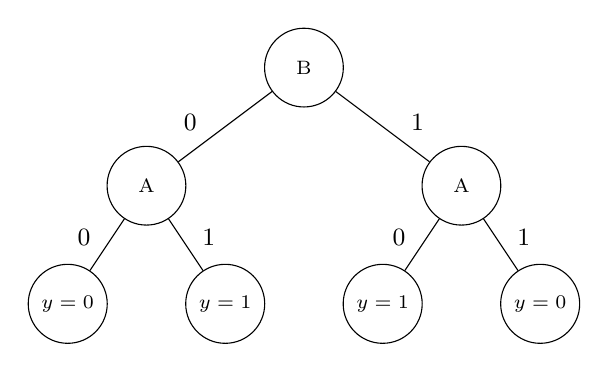
\begin{tikzpicture}[
          level 1/.style={sibling distance=40mm},
          level 2/.style={sibling distance=20mm},
          split/.style={draw, circle, minimum width=10mm, font=\scriptsize},
          leaf/.style={draw, circle, minimum width=10mm, font=\scriptsize},
          edge from parent/.style={draw, -},
          edge label/.style={font=\small, pos=0.7}
        ]
          \node[split] {B}
            child {
              node[split] {A}
              child {
                node[leaf] {$y=0$}
                edge from parent node[edge label, above left] {0}
              }
              child {
                node[leaf] {$y=1$}
                edge from parent node[edge label, above right] {1}
              }
              edge from parent node[edge label, above left] {0}
            }
            child {
              node[split] {A}
              child {
                node[leaf] {$y=1$}
                edge from parent node[edge label, above left] {0}
              }
              child {
                node[leaf] {$y=0$}
                edge from parent node[edge label, above right] {1}
              }
              edge from parent node[edge label, above right] {1}
            };
        \end{tikzpicture}
        \caption{Tree splits on B first, then A}
      \end{subfigure}
      \caption{Two functionally equivalent decision trees that implement the XOR function: $y = A \oplus B$}
    \end{figure} 
  \end{example}

  Therefore, there is repetition in our model space, and our misclassification loss will treat them equally. Even though they are functionally the same, it doesn't make them \textit{practically} equal. In reality, with missing data, we would like the path to our leaves---the final decisions---to be short as possible. Therefore, we may not need to use every covariate to reach a decision. If we can avoid the uncertain covariates (e.g. ones with more missing values or noise), then we can get a more robust decision tree. 

  \begin{example}[Robust Decision Tree without Always Querying Covariate $A$]
    We can see that the two decision trees are functionally the same. 
    \begin{equation}
      f(x) = \begin{cases} 
        0 & \text{ if } (A, B, C) = (0, 0, 0) \\
        0 & \text{ if } (A, B, C) = (0, 0, 1) \\
        1 & \text{ if } (A, B, C) = (0, 1, 0) \\
        1 & \text{ if } (A, B, C) = (0, 1, 1) \\
        0 & \text{ if } (A, B, C) = (1, 0, 0) \\
        1 & \text{ if } (A, B, C) = (1, 0, 1) \\
        0 & \text{ if } (A, B, C) = (1, 1, 0) \\
        1 & \text{ if } (A, B, C) = (1, 1, 1)
      \end{cases}
    \end{equation}

    Note that the right tree can do the same as the left tree, but in some cases it does not need to query $A$ at all. Therefore, in some cases, we can reach a decision even when $A$ is missing.

    \begin{figure}[H]
      \centering
      \begin{subfigure}[b]{0.38\textwidth}
        \centering
        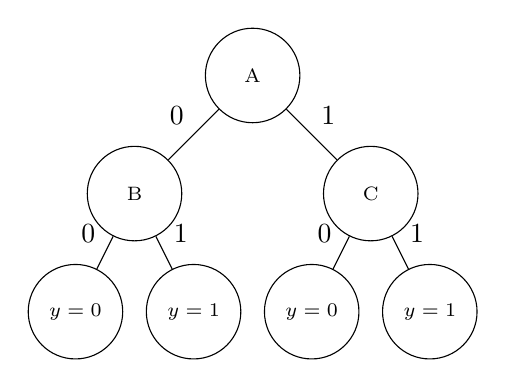
\begin{tikzpicture}[
          level 1/.style={sibling distance=30mm},
          level 2/.style={sibling distance=15mm},
          split/.style={draw, circle, minimum width=12mm, font=\scriptsize},
          leaf/.style={draw, circle, minimum width=12mm, font=\scriptsize},
          edge from parent/.style={draw, -}
        ]
          \node[split] {A}
            child {
              node[split] {B}
              child {
                node[leaf] {$y=0$}
                edge from parent node[above left] {0}
              }
              child {
                node[leaf] {$y=1$}
                edge from parent node[above right] {1}
              }
              edge from parent node[above left] {0}
            }
            child {
              node[split] {C}
              child {
                node[leaf] {$y=0$}
                edge from parent node[above left] {0}
              }
              child {
                node[leaf] {$y=1$}
                edge from parent node[above right] {1}
              }
              edge from parent node[above right] {1}
            };
        \end{tikzpicture}
      \end{subfigure}
      \hfill 
      \begin{subfigure}[b]{0.58\textwidth}
        \centering
        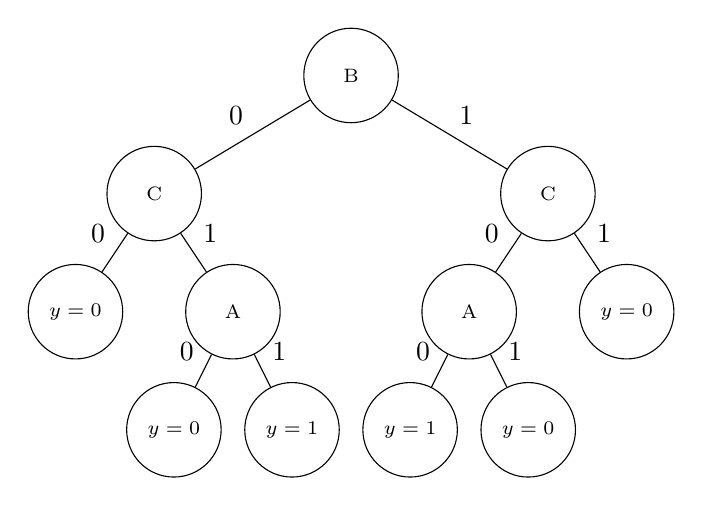
\begin{tikzpicture}[
          level 1/.style={sibling distance=50mm},
          level 2/.style={sibling distance=20mm},
          level 3/.style={sibling distance=15mm},
          split/.style={draw, circle, minimum width=12mm, font=\scriptsize},
          leaf/.style={draw, circle, minimum width=12mm, font=\scriptsize},
          edge from parent/.style={draw, -}
        ]
          \node[split] {B}
            child {
              node[split] {C}
              child {
                node[leaf] {$y=0$}
                edge from parent node[above left] {0}
              }
              child {
                node[split] {A}
                child {
                  node[leaf] {$y=0$}
                  edge from parent node[above left] {0}
                }
                child {
                  node[leaf] {$y=1$}
                  edge from parent node[above right] {1}
                }
                edge from parent node[above right] {1}
              }
              edge from parent node[above left] {0}
            }
            child {
              node[split] {C}
              child {
                node[split] {A}
                child {
                  node[leaf] {$y=1$}
                  edge from parent node[above left] {0}
                }
                child {
                  node[leaf] {$y=0$}
                  edge from parent node[above right] {1}
                }
                edge from parent node[above left] {0}
              }
              child {
                node[leaf] {$y=0$}
                edge from parent node[above right] {1}
              }
              edge from parent node[above right] {1}
            };
        \end{tikzpicture}
      \end{subfigure}
      \caption{Credits to \cite{2025mctavish}.}
    \end{figure}
  \end{example}
  
  In 2025, McTavish showed an algorithm of finding such trees \cite{2025mctavish}. 

